\section{Position Based Dynamics} \label{ch2:pbd} %название по-русски
	Предложенный в 2007 году алгоритм Position Based Dynamics\cite{pbd} является оснополагающим для большинства современных алгоритмов симуляции тканей. Рассмотрим принципы работы и математические модели, лежащие в основе данного метода.
	
	В рамках предложенной математической модели, любое симулируемое тело представляет собой набор из $N$ частиц, соединенных $M$ ограничениями. При этом \textbf{состояние частицы $i$} характеризуется следующими параметрами:
	\begin{enumerate}[1.]
		\item Положение частицы (в момент времени $t$) $p_i(t)$
		\item Обратная масса $im_i = 1/m_i$
	\end{enumerate}
	
	Стоит отметить две важные особенности рассматриваемой математической модели. Во-первых, размер частицы считается пренебрежимо малым по отношению к размеру всего тела. Во-вторых, для описания состояния частицы не используются скорость и ускорение данной частицы (в отличие от методов симуляции, используемых для обработки физического взаимодействия абсолютно твердых тел).
	
	Под \textbf{ограничением $j$} понимается набор из:
	\begin{enumerate}[1.]
		\item Размерности ограничения (количество затрагиваемых частиц) $n_j$
		\item Функции $C_j: \mathbb{R}^{n_j}->\mathbb{R}$
		\item Набор индексов частиц, к которым применяется данное ограничение $\{i_1, i_2, ..., i_{n_j}\}, i_k \in [1, ..., N]$
		\item Параметр жесткости $k_j \in [0...1]$
		\item Тип \say{равенство} или \say{неравенство}
	\end{enumerate}
	
	Будем считать, что ограничение $j$ типа \say{равенство} выполнено (удовлетворено), когда выполняется следующее условие:
	\begin{equation} \label{eq:constraint-eq}
		C_j(p_{i_1}, p_{i_2}, ..., p_{i_{n_j}}) = 0
	\end{equation} 
	
	Если же ограничение $j$ имеет тип \say{неравенство}, тогда будем считать, что оно выполнено (удовлетворено), когда выполняется:
	\begin{equation} \label{eq:constraint-neq}
		C_j(p_{i_1}, p_{i_2}, ..., p_{i_{n_j}}) \ge 0
	\end{equation} 
	
	В качестве примера можно привести ограничение \say{пружина}, использующееся для симуляции ткани. Функция $C_j$ такого ограничения будет выглядеть следующим образом:
	\begin{equation} \label{eq:constraint-spring}
		C_j(p_{i_1}, p_{i_2}) = |p_{i_1} - p_{i_2}| - d
	\end{equation} 
	
	В этом выражении переменная $d$ обозначает длину \say{пружины} в состоянии покоя. В дальнейшей работе будут рассматриваться только ограничения вида \say{равенство}, однако ограничение типа \say{неравенство} может быть приведено к ограничению типа \say{равенство} при помощи построения новой функции ограничения $C^{'}_{j} = max(0, C_j)$.
	
	Тогда, если частицы и их ограничения заданы вышеописанным способом, алгоритм PBD будет представляться следующим образом (\firef{alg:PositionBasedDynamics}).
	
	\begin{algorithm} %[h]
		\SetKwFunction{algoPBDPseudocode}{} 
		\SetKwProg{myalg}{Algorithm}{}{} %write in 2nd agrument <<Algorithm>>, <<Procedure>> etc
		\nonl\myalg{\algoPBDPseudocode}{
			\KwInput{
				время шага симуляции $\Delta t$,
				количество итераций $solverIteration$,
				текущее состояние частиц,
				предыдущее состояние частиц,
				ограничения,
				функция суммы внешних сил от положения $f_{ext}(p)$
			}
			\KwOutput{положение частиц спустя заданное время $\{p_i(t + \Delta t)\}_N$}
			
			\For {$i \in 1..N$ \label{step:pbd-solver-integrate}}{
				$v_i = \frac{p_i(t) - p_i(t -\Delta t)}{\Delta t} + \Delta t * im_i * f_{ext}(p_i)$;
				
				$p^*_i = p_i(t) + v_i * \Delta t $;
			}
			
			\For{$k \in 1..solverIteration$ \label{step:pbd-solver-loop}}{
				$p^*_1, ..., p^*_N = projectConstraints(p^*_1, ..., p^*_N)$;
			}
			
			\For {$i \in 1..N$ \label{step:pbd-solver-save}}{
				$p_i(t + \Delta t) = p^*_i$;
			}
		}		
		\caption{Псевдокод алгоритма Position Based Dynamics}\label{alg:PositionBasedDynamics}
	\end{algorithm}
	\FloatBarrier
	
	Как можно заметить, данный алгоритм является итеративным и определяет новое состояние тела из текущего состояния и величины прошедшего времени. Начинается алгоритм с предсказания новых положений частиц путем численного интегрирования уравнения перемещения частицы методом Стёрмера-Верле\cite{verlet1967computer} (строка \ref{step:pbd-solver-integrate}). Данный метод был выбран потому, что для него достаточно только одного предыдущего значения, а также он является более устойчивым, чем метод Эйлера. Далее (строка \ref{step:pbd-solver-loop}) несколько раз (указанное в аргументе $solverIteration$) запускается алгоритм $projectConstraints$, который модифицирует предсказанные положения частиц таким образом, чтобы приблизится к выполннению всех поставленных ограничений. Затем (строка \ref{step:pbd-solver-save}) положения частиц на момент времени $t + \Delta t$ принимаются равными предсказанным позициям.
	
	Для того, чтобы описать принцип работы алгоритма $projectConstraints$, необходимо найти способ решать такую задачу для одного ограничения. Для этого возьмем произвольное ограничение и обозначим функцию этого ограничения $C$. Поставим задачу найти вектор $\Delta p$ такой, что:
	\begin{equation}
		C(p + \Delta p) = 0
	\end{equation}
	
	Для этого достаточно разложить данное равенство в ряд Тейлора:
	\begin{equation}
		C(p + \Delta p) \approx C(p) + \Delta p * \nabla_{p} C(p) = 0
	\end{equation}
	
	Преобразовав полученное равенство и выделив множитель $scaleFactor$, общий для всех связанных данным ограничением частиц, получим:
	\begin{equation} \label{eq:delta_p_scaleFactor}
		scaleFactor = -\frac{C(p)}{|\nabla C(p)|^2}
	\end{equation}
	\begin{equation} \label{eq:delta_p_pbd}
		\Delta p_i = scaleFactor* \nabla_{p_i} C(p)
	\end{equation}
	
	Таким образом, используя выражение \ref{eq:delta_p_pbd}, мы для каждой связанной ограничением частицы можем найти смещение, необходимое для удовлетворения данного ограничения, но только в случае, если массы частиц равны между собой. Иначе требуется воспользоваться приведенным ниже выражением \ref{eq:delta_p_scaleFactor_2}:
	
	\begin{equation} \label{eq:delta_p_scaleFactor_2}
		scaleFactor = -\frac{1}{\sum_l im_l} \frac{C(p)}{|\nabla C(p)|^2}
	\end{equation}
	\begin{equation} \label{eq:delta_p_pbd_2}
		\Delta p_i = im_i * scaleFactor * \nabla_{p_i} C(p)
	\end{equation}

	Стоит отметить, что при значении $im_i = 0$ (соответствует бесконечной массе) не только вектор смещения $\Delta p_i = 0$, но и внешние силы при интеграции методом Стёрмера-Верле (\firef{alg:PositionBasedDynamics}) не будут влиять на положение вершины. Это означает, что таким образом можно \say{закреплять} такие вершины в пространстве, или \say{прикреплять} к другим симулируемым физическим телам.
	
	\begin{algorithm} %[h]
		\SetKwFunction{solveConstraint}{} 
		\SetKwProg{myalg}{Algorithm}{}{}
		\nonl\myalg{solveConstraint}{
			\KwInput{
				размерность ограничения $n$,
				функция ограничения $C$, 
				текущие положения частиц $\{p_i\}_n$,
				обратные массы частиц $\{im_i\}_n$
			}
			\KwOutput{вектора смещения частиц $\{\Delta p_i\}_n$ для удолветворения заданному ограничению}
						
			$scaleFactor = {C(p_1, ...)} / {\sum_{i}(im_i *|\nabla_{p_i} C(p_1, ..., p_{n})|^2)}$;
			
			\lFor {$i \in 1..n$}{
				$\Delta p_i = -scaleFactor * im_i * \nabla_{p_i} C(p_1, ..., p_{n})$
			}
		}
		\caption{Псевдокод алгоритма solveConstraint}\label{alg:SolveConstraint}
	\end{algorithm}
	\FloatBarrier
	
	Таким образом получаем алгоритм $solveConstraint$ (\firef{alg:SolveConstraint}) для решения задачи в случае одного ограничения. Для того, чтобы решить задачу для набора ограничений, авторами было предложено 2 алгоритма. 
	
	Первый (\firef{alg:projectConstraintsJacobi}), по словам авторов, основан на методе Якоби для решения СЛАУ, хотя функции ограничений не всегда являются линейными. Идея данного алгоритма заключается в том, чтобы для каждого ограничения вычислить смещения соответствующих вершин и сохранить их во временную переменную. Затем для каждой частицы прибавить к её положению значение суммарного смещения, сохранённое во временной переменной, умноженный на некоторую скалярную константу $\gamma$.
	
	\begin{algorithm} %[h]
		\SetKwFunction{projectConstraintsJacobi}{} 
		\SetKwProg{myalg}{Algorithm}{}{} %write in 2nd agrument <<Algorithm>>, <<Procedure>> etc
		\nonl\myalg{projectConstraintsJacobi}{
			\KwInput{
				константа $\gamma$,
				ограничения,
				текущее состояние частиц
			}
			\KwOutput{новые положения частиц $\{p^*_i\}_N$}
			
			\lFor {$i \in 1..N$} {
				$o_i = 0$
			}
			
			\For {$j \in 1..M$}{
				$tmp = solveConstraint(n_j, C_j, p_{i_{1}}, ..., p_{i_{n_j}}, im_{i_{1}}, ..., im_{i_{n_j}})$;
				
				\For {$l \in 1..n_j$} {
					$o_{i_l} = o_{i_l} + k_j * tmp_{l}$
				}
			}
			
			\lFor {$i \in 1..N$}{
				$p^*_i = p_i + \gamma * o_i$
			}
		}
		\caption{Псевдокод алгоритма projectConstraints использующего метод Якоби}\label{alg:projectConstraintsJacobi}
	\end{algorithm}
	\FloatBarrier

	Второй (\firef{alg:projectConstraintsGauss}), по словам авторов, основан на методе Гаусса-Зейделя для решения СЛАУ. Данный метод отличается от предыдущего тем, что смещения применяются к частицам сразу, а не накапливаются.

	\begin{algorithm} %[h]
	\SetKwFunction{projectConstraintsGauss}{} 
	\SetKwProg{myalg}{Algorithm}{}{} %write in 2nd agrument <<Algorithm>>, <<Procedure>> etc
	\nonl\myalg{projectConstraintsGauss}{
		\KwInput{
				ограничения,
				текущее состояние частиц
		}
		\KwOutput{новые положения частиц $\{p^*_i\}_N$}
		
		\For {$j \in 1..M$}{
			$tmp = solveConstraint(n_j, C_j, p_{i_{1}}, ..., p_{i_{n_j}}, im_{i_{1}}, ..., im_{i_{n_j}})$;
			
			\For {$l \in 1..n_j$} {
				$p^*_i = p_i + k_j * tmp_{l}$;
			}
		}
		
	}
	\caption{Псевдокод алгоритма projectConstraints использующего метод Гаусса-Зейделя}\label{alg:projectConstraintsGauss}
	\end{algorithm}
	\FloatBarrier
	
	Как можно заметить, оба алгоритма ориентируются на итеративные алгоритмы решения СЛАУ. Для выбора между этими двумя алгоритмами, авторы оригинальной статьи поставили мысленный эксперимент (\firef{fig:jacobi_vs_gauss}):
	
	\begin{enumerate}[1.]
		\item Рассматриваются три частицы $p_1, p_2, p_3$. Частицы $p_1, p_3$ закреплены в пространстве.
		\item Рассматривается два ограничения \say{пружина}: $C_1(p_1, p_2)$ с длиной покоя $l_1$ и $C_2(p_2, p_3)$ с длиной покоя $l_2$.
		\item Исходя из приведенного на рисунке положения частиц, видно, что оптимальным положением частицы $p2$ является точка пересечения пунктирных дуг, имеющих радиусы $l_1$ и $l_2$.
		\item Проводится одна итерация алгоритмом, основанным на методе Якоби, и одна итерация алгоритмом, основанным на методе Гаусса-Зейделя
		\item В результате поставленного эксперимента можно наблюдать, что первый алгоритм сходится медленнее чем второй.
	\end{enumerate}
		
	\begin{figure}[h!] 
		\center
		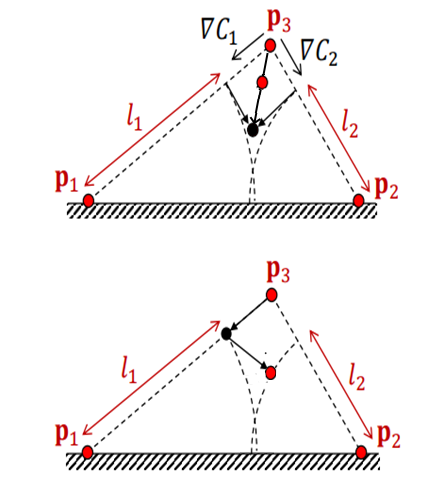
\includegraphics [scale=0.65] {my_folder/images//jacobi_vs_gauss}
		\caption{Эксперимент поставленный авторами статьи.\newline На верхнем изображении представлен результат первой итерации алгоритмом основанным на методе Якоби, на нижнем изображении результат первой итерации алгоритмом основанным на методе Гаусса-Зейделя}
		\label{fig:jacobi_vs_gauss}  
	\end{figure}
	
	Помимо мысленных экпериментов, авторами были поставлены и численные эксперименты с использованием компьютера.Согласно полученным ими результатам, первый алгоритм действительно сходится медленнее, для его реализации требуется выделение дополнительной памяти и подбор значения константы $\gamma$. В качестве преимуществ авторы отмечают возможность и простоту параллельной реализации. С другой стороны, алгоритм, основанный на методе Гаусса-Зейделя, сходится быстрее, его реализация не требует дополнительного объема памяти, но полученный результат будет зависеть от порядка обхода ограничений. Возможность параллельной реализации данного алгоритма зависит от выбора порядка обхода ограничений.

%% Вспомогательные команды - Additional commands
%
%\newpage % принудительное начало с новой страницы, использовать только в конце раздела
%\clearpage % осуществляется пакетом <<placeins>> в пределах секций
%\newpage\leavevmode\thispagestyle{empty}\newpage % 100 % начало новой страницы